
%
% # INTRODUCTION:
%
% This write up is for Lab1: Lab Introduction.
%
% Specifically this was used for the class Logic Design Fundamentals (EECE 144)
% taught by Kurtis Kredo [http://www.ecst.csuchico.edu/~kkredo/]
% during the Fall 2011 semester at CSU Chico [www.csuchico.edu].
% 
% ## LaTeX
%
% This file is written for LaTeX [http://www.latex-project.org/]
% which is used to process this file in to a completely formatted
% document.
%
% If you are unfamiliar with LaTeX it can seem daunting at first
% (as with anything new) but there are many benefits.
% Imagine writing a document in Word except without
% having to worry about the tedious things such as line breaks,
% indentation, table of contents, appendices, font styles,
% heading sizes, citations/references, page numbers.
% LaTeX lets you focus on the content without
% worrying about the tedious details.  It is also excellent for
% producing mathematical formulas.
% 
% If you are collaborating with someone else you can simply edit
% the sections and paragraphs in this file as needed.
%
% To process this file use a command such as 'rubber'.
%
%   bash$ rubber skel.tex
%   (output to skel.dvi)
%   bash% rubber --pdf skel.tex
%   (output to skel.pdf)
%
% # AUTHORS (of this template):
%
%   Jeremiah Mahler <jmmahler@gmail.com>
%   https://www.google.com/profiles/jmmahler#about 
%
% # COPYRIGHT:
%
%   Copyright (C)  2011 Jeremiah Mahler <jmmahler@gmail.com>.
%   Permission is granted to copy, distribute and/or modify this document
%   under the terms of the GNU Free Documentation License, Version 1.3
%   or any later version published by the Free Software Foundation;
%   with no Invariant Sections, no Front-Cover Texts, and no Back-Cover Texts.
%   A copy of the license is included in the file "fdl-1.3.txt".
%

\documentclass[12pt]{article}
%\documentclass[10pt]{article}

%\usepackage{mslapa}
\usepackage{hyperref}
\usepackage{amsmath}
\usepackage{graphicx}
\usepackage{ulem}
\usepackage{vmargin}
\usepackage{tabularx}
\usepackage{sectsty}
\usepackage{pbox}
\usepackage{bigstrut}
\usepackage{enumerate}

\setpapersize{USletter}
\sectionfont{\normalsize}

\begin{document}


% {{{ Cover Page

\centerline{\bf EECE 144}
\centerline{\bf Fall 2011}
\centerline{\bf}
\centerline{\bf Lab Report \#1}
\centerline{\bf Section 4}
\centerline{\bf 9/7/2011}

% signature area
% TODO - how to get more vertical space from \bigstrut?
\begin{center}
\begin{tabularx}{\textwidth}[b]{X X l}
Submitted by: & & \\
Signature & Printed Name & Date \\
\hline
\multicolumn{1}{|X|}{} & \multicolumn{1}{|l|}{\bigstrut \bf Jeremiah Mahler} & \multicolumn{1}{|l|}{\bf Sep 7, 2011} \\
\hline
\multicolumn{1}{|X|}{} & \multicolumn{1}{|l|}{\bigstrut \bf Marvanee Johnson} & \multicolumn{1}{|l|}{\bf Sep 7, 2011} \\
\hline
\end{tabularx}
\end{center}
% }}}

\section{Description/Objectives}

The objective of this lab is to introduce a student to
the essential lab equipment that will be used in subsequent labs.
Specifically the digital multimeter, voltage supply, and digital simulation
software are introduced.

\section{Procedure}

The multimeter is used primarly to measure voltage.
There are two multimeters available and they differ in
the resolution of their measurement.
One has a resolution of 0.01 volts whereas the other has a resolution
of 0.0001 volts.
And there is a voltage supply which provides a voltage across
different pairs of terminals in either 5 volts or 12 volts.
To test the operation of the multimeter and voltage supply the test
leads of the meter are connected to the voltage supply and the voltage
is read.

Logisim \cite{LOGISIM} is software that can be used to simulate digital
circuits.
To introduce the student to this software they should create a basic circuit
with a few elements.
A good example is to add one AND gate and one OR gate (see Figure \ref{fig:logisim}).
Then input pins can be connected to the terminals along with an output pin.
Then in simulation mode (as opposed to edit mode) the pins can be set hi/low
and the output behaviour can be verified.

% include screenshot
\begin{figure}[!hbtp]
\center
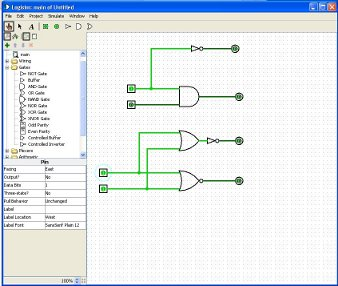
\includegraphics[scale=1.0]{logisim-02}
\caption{Logisim running under Windows with several gates: AND, OR, NOT.}
\label{fig:logisim}
\end{figure}

\clearpage % flush all the figures

\section{Observations}

Connecting the meter to the voltage supply resulted a voltage reading
as expected.
And if the terminals were reversed the result was a negative value.
The labels on the voltage supply suggested the readings should be
exactly 5 volts or 12 volts but the actual measurements were quite different.
On the 5 volt terminals the lower resolution meter read 5.15 volts and
the higher resolution meter read 5.1535 volts.
On the 12 volt terminals the lower resolution meter read 12.47 volts and
the higher resoltion meter read 12.4723 volts.

The simulation of the AND, OR and NOT gates in Logisim behaved as expected
and followed their truth table values (Figure \ref{fig:gatett}).

\begin{figure}[!hbt]

\center
\begin{tabular}{c c c}  % outer alignment table

\begin{tabular}[t]{| l | l | l |}
\hline
\multicolumn{3}{| l |}{AND} \\
\hline
A & B & out \\
\hline
0 & 0 & 0 \\
\hline
0 & 1 & 0 \\
\hline
1 & 0 & 0 \\
\hline
1 & 1 & 1  \\
\hline
\end{tabular}

& 

\begin{tabular}[t]{| l | l | l |}
\hline
\multicolumn{3}{| l |}{OR} \\
\hline
A & B & out \\
\hline
0 & 0 & 0 \\
\hline
0 & 1 & 1 \\
\hline
1 & 0 & 1 \\
\hline
1 & 1 & 1  \\
\hline
\end{tabular}

&

\begin{tabular}[t]{| l | l |}
\hline
\multicolumn{2}{| l |}{NOT} \\
\hline
A & out \\
\hline
0 & 1 \\
\hline
1 & 0 \\
\hline
\end{tabular}

\end{tabular} % end outer alignment table

\caption{Truth tables for AND, OR, and NOT gates.}
\label{fig:gatett}
\end{figure}

%\clearpage

\section{Conclusion}

This lab was a success in introducing a student to the basic equipment
in the lab.
The meter and voltage supply read voltages as expected but their readings
were significantly biased causing the values to be larger then expected.
The digitial circuit simulator, Logisim, also worked as expected and the
truth tables for AND, OR and NOT were confirmed.

% flush all the figures
%\clearpage

%\pagebreak
\renewcommand*{\refname}{}
\section{References}
%\bibliographystyle{plain}
%\bibliographystyle{mslapa}
\bibliographystyle{ieeetr}
\bibliography{main}  % main.bib

% Appendix (if needed)

\end{document}

% vim:foldmethod=marker
